\documentclass{article}
\usepackage{amsmath}
\usepackage{amssymb}
\usepackage{quiver}
\usepackage{tikz-cd}
\usepackage[a4paper, margin=1in]{geometry}

\usepackage{amsthm}
\newtheorem{lemma}{Lemma}
\newtheorem{prop}{Proposition}

\newcommand{\C}{\mathbb{C}}
\newcommand{\Z}{\mathbb{Z}}
\newcommand{\R}{\mathbb{R}}
\newcommand{\bP}{\mathbb{P}}
\newcommand{\OO}{\mathcal{O}}
\newcommand{\sslash}{\mathbin{/\mkern-4mu/}}
\newcommand{\Spec}{\text{Spec}}
\newcommand{\Proj}{\text{Proj}}
\newcommand{\m}{\mathfrak{m}}
\newcommand{\fk}{\mathfrak{k}}
\newcommand{\Rep}{\mathrm{Rep}}
\newcommand{\Hom}{\text{Hom}}
\newcommand{\cL}{\mathcal{L}}
\newcommand{\cA}{\mathcal{A}}
\newcommand{\Tr}{\mathrm{Tr}}
\newcommand{\p}{\mathfrak{p}}
\newcommand{\cF}{\mathcal{F}}
%

\begin{document}
\noindent PMATH 965 A2\\
Kaleb R, 20658568 \vspace{1em}
%% 
%% QUESTION 1
%%

\noindent \textbf{Question 1} \\
Let $K = U(n)$ acting on $X=M(n,k)$ by left multiplication. For any $A,B \in \Gamma(TM(n,k))$, define a symplectic form on $X$ by
$$\omega(A,B) = \frac{1}{2i}\Tr(A^\dagger B - B^\dagger A).$$
Then I claim that $\mu:X\to \mathfrak{u}(n)^\ast$, defined by
$$\mu(x) = \left(\alpha \to \left(\frac{1}{2i}\Tr\left(x^\dagger \alpha^\dagger x\right)\right)\right)$$
is a moment map for the $U(n)$ action on $(X,\omega)$. First we check it is equivariant. Suppose $U\in U(n)$ and $\alpha \in \mathfrak{u}(n)$.
\begin{align*}
	\mu(U\cdot x)(\alpha) &= \frac{1}{2i}\Tr(x^\dagger U^\dagger \alpha^\dagger Ux)\\
	&= \frac{1}{2i}\Tr\left((U^\dagger \alpha U) x\right)\\
	&= \mu(x)(U^\dagger\alpha U)
\end{align*}
Now since $U$ is unitary, $U^\dagger = U^{-1}$, so this becomes
\begin{align*}
	\mu(U\cdot x)(\alpha)&= \mu(x)(U^{-1}\alpha U)\\
	&= \mu(x)(U\cdot \alpha).
\end{align*}
Hence $\mu$ is $U(n)$-equivariant. Next we check that 
\begin{equation}
	\label{e:cond2}
	d\left(\mu(x)(A)\right) = \omega_x(X_\alpha, A).
\end{equation}
First, we can find a more explicit formula for $X_\alpha$ since $U(n)$ is a matrix Lie group:
$$X_\alpha(x) := \frac{d}{dt}|_{t=0} e^{t\alpha}\cdot x = \alpha x$$
Then the right side of equation (\ref{e:cond2}) is
\begin{align*}
	\omega_x(X_\alpha, A) &= \frac{1}{2i}\Tr(A^\dagger X_\alpha - X_\alpha^\dagger A)\\
	&= \frac{1}{2i}\Tr(A^\dagger \alpha x - x^\dagger \alpha^\dagger A).
\end{align*}
For the left side we first compute
$$\mu(x)(\alpha) = \frac{1}{2i}\Tr(x^\dagger \alpha x)$$
To take $d$ of this, we consider a path $x(t)=x+At$ in $U(n)$, for an arbitrary $A\in\Gamma(TX)$. Then 
\begin{align*}
	(d\mu(x)(\alpha))(A) &= \frac{1}{2i}\frac{d}{dt}|_{t=0} \Tr(x(t)^\dagger \alpha x(t))\\
	&= \frac{1}{2i}\Tr(A^\dagger \alpha x + x^\dagger \alpha A)\\
	&= \frac{1}{2i}\Tr(A^\dagger \alpha x - x^\dagger \alpha^\dagger A).
\end{align*}
Where in the last step we used that since $\alpha \in \mathfrak{u}(n)$, $\alpha^\dagger = -\alpha$. Thus the left and right hand sides are equal, and $\mu$ is indeed a moment map. \vspace{1em}

Now, we can form the symplectic quotient. Fix some $\eta \neq 0$ in $\mathfrak{u}^\ast$. We identify $\mathfrak{u}^\ast$ with $\mathfrak{u}$ by the map
\begin{equation}
	B \to (A\to \Tr(B^\dagger A)).
\end{equation}
Composing this with our moment map, we can view $\mu:X\to \mathfrak{u}(n)$ given by
$$\mu(x) = \frac{1}{2i}xx^\dagger.$$
Then let $\eta$ be a regular point of $\mu$ in $ \mathfrak{u}(n)$, say (up to redefining $\mu$), $\eta=\frac{1}{2i}I_n$, the identity matrix. The symplectic quotient is defined to be
$$X\sslash K := \mu^{-1}(\eta)/U(n).$$
To compute this, I claim first that every matrix in $\mu^{-1}(\eta)$ has rank $n$. If $x$ has rank less than $n$, then $xx^\dagger$ has rank less than $n$ and hence cannot be $I_n$. Furthermore, if $xx^\dagger = I_m$ then $x$ must be "unitary" i.e. its $n$ linearly independent columns form an orthonormal basis of $\C^n$. These $n$ columns define an $n$-dimensional subspace of $\C^k$. Two such matrices $x$ and $y$ yield the same $n$-dimensional subspace exactly when there is a change-of-basis matrix between the columns. This matrix will be unitary since the sets of columns are orthonormal. Hence we finally arrive at:
$$X\sslash K = \{n-\text{dimensional subspaces of }\C^k\} = \mathrm{Gr}(n,k).$$

\pagebreak

%%
%%QUESTION 2
%%
\noindent \textbf{Question 2} \\
 Let $K = \C^\ast$ and let it act on $\C^{m+1}$ via weight matrix $A=[a_1,...,a_m,-d]$, with gcd$(a_1,...,a_m)=1$, $a_i | d$ and $a_i,d > 0$ integers. \vspace{1em}

\noindent \textbf{a)} Let $\omega = 1$. To compute the semi-stable locus, we will use the proposition which tells us
\begin{equation}
    V_\omega^{ss} = \bigcup_{I\in\cA_\omega} (\C^\ast)^I \times \C^{\overline{I}}.
\end{equation}
We need to find $\cA_\omega$. Since all the $a_i$ are positive integers, $1$ is in any rational cone containing any of the $a_i$, but not the cone over just $-d$. Hence $\cA_\omega = \left\{I\subset [m+1] ~|~ I\neq \{m+1\}\right\}.$ This tells us that the semi-stable locus is
\begin{equation}
    V_\omega^{ss} = \{z = (z_1,...,z_{m+1}) \in \C^{m+1} ~|~ \exists i\neq m+1 \text{ s.t. } z_i \neq 0 \} = (\C^m - \{0\})\times \C.
\end{equation}
Now we can take the $\C^\ast$ quotient. We will adopt the viewpoint that we have a trivial line bundle over $(\C^m-\{0\})$ which we are quotienting. The factor of $(\C^m-\{0\})/\C^\ast$ with weights $[a_1,...,a_m]$ gives exactly the definition of $\bP(a_1,...,a_m)$. The "sections" of the trivial line bundle that descend are those families of points $(z_1,...,z_m,l)\in V^{ss}_\omega$ for which
\begin{equation}
    t^{-d} l(t\cdot z) = l(z).
\end{equation}
These are precisely the degree-d homogeneous functions with respect to the weighted grading on $\C[x_1,...,x_m]$. Hence we see that our quotient is the total space of $\mathcal{O}(d)$ over $\bP(a_1,...,a_m)$. \vspace*{1em}

\noindent \textbf{b)} Now let $\omega = -1$. Again we find the anti-cones; this time an anticone will contain $\omega$ if and only if $-d$ is one of the generating rays. This is because the rest of the weights $a_1,...,a_m$ are positive and hence any cones they define consist only of positive numbers. The semi-stable locus is therefore
\begin{equation}
    V^{ss}_\omega = \{(z_1,...,z_m)\in \C^{m+1} ~|~ z_{m+1}\neq 0 \} = \C^m \times \C^\ast.
\end{equation}
Next we try to take the $\C^\ast$ quotient. We will adopt the viewpoint that we have a trivial $\C^m$ bundle over $(\C^\ast)$ that we are quotienting. The quotient of $\C^\ast$ by $\C^\ast$ with weight $d$ gives one point, because
$$\sqrt[d]{\frac{w}{z}}^d z = w$$
so $z\sim w$ for all $z,w\in \C^\ast$. The sections of the bundle that descend are those semi-stable points for which
$$(t^{a_1} s_1(t\cdot z_{m+1}),...,t^{a_m}s_m(t\cdot z_{m+1})) = (s_1(z_{m+1}),...,s_m(z_{m+1})).$$ 
I.e. we have $t^{a_i}s_i(t\cdot z_{m+1}) = s_i(z_{m+1})$ is a degree $a_i$ homogeneous polynomial, so our quotient is 
$\bigoplus_{i=1}^m \mathcal{O}(a_i)$ over a single point. There is only one homogeneous polynomial of degree $a_i$ in one variable ($z^{a_i}$), so our quotient is isomorphic to the vector space $\C^m$.

\pagebreak

%%
%% QUESTION 3
%%
\noindent \textbf{Question 3} \\
\textbf{a)} Let $v$ be a vertex of $P$. Then $v$ is the intersection of $n$ facets of $P$, say $v = \bigcap_{i\in I} F_i$. These facets have inward facing vectors $\{\rho_i\}_{i\in I}$. Thus, we can associate an $n$-dimensional cone $\sigma$ to $v$: the cone over $\{\rho_i\}_{i\in I}$. \vspace{1em }

Let $U_\sigma = \Spec(\C[\sigma^\vee \cap M])$. A point $\p$ in $U_\sigma$ defines a map $\C[\sigma^\vee \cap M] \to \C$ by quotienting. By thinking of $\sigma^\vee\cap M \subset \C[\sigma^\vee \cap M]$ we can also consider $\p$ to be a map $\sigma^\vee\cap M\to \C$. Similarly, an element of the torus $T=\Spec(\C[M])$ is a map $M\to \C^\ast$. In this view, the torus action $T$ on $U_\sigma$ is given by the map $t\cdot \p$ defined to be
$$t\cdot \p (m) = t(m)\p(m).$$
Therefore a fixed point is an ideal $\p$ in $U_\sigma$ for which $\p(m) = t(m)\p(m)$ for all $m\in \sigma^\vee\cap M$. Define a map $f:\sigma^\vee\cap M\to \C$ by
$$f(m) = \begin{cases}
	0, & m\neq 0\\
	1, & m=0.
\end{cases}$$
For $m\neq 0$ we have $f(m) = 0 = t(m)f(m)$, and for $m=0$ we have $f(m)=1=t(m)f(m)$. The latter is because $t(0)$ must be $1$ as $t$ is a homomorphism. Finally, we must show that this map $f$ indeed defines a point $\p \in U_\sigma$; i.e. that $f$ is a homomorphism. Suppose $m_1,m_2\in \sigma^\vee\cap M$. We want
$$f(m_1 + m_2) = f(m_1)f(m_2)$$
If $m_1 + m_2 \neq 0$ then this holds. Suppose $m_1+m_2 = 0$. Then either $m_1=m_2=0$, in which case the equation holds again, or $m_1=-m_2$. If $m_1=-m_2$ non-zero then $\sigma^\vee$ is not strongly convex. This contradicts the fact that $\sigma$ is dimension $n$. Hence $f$ is a homomorphism and it defines a fixed point in $U_\sigma$. Since $f$ sends all the non-constant maps in $\C[\sigma^\vee\cap M]$ to 0, $\p$ is defined by the maximal ideal $\p = \langle \rho_1,...,\rho_n \rangle$. \vspace{2em}

\noindent \textbf{b)} Let $v = \bigcap_{i\in I} F_i$ with $F_i$ defined by inward facing normal $\rho_i$. Let $u_1,...,u_n$ be the inward facing edges of $v$. If $u_j \in F_i$, then $\langle \rho_i, u_j \rangle = 0$. This implies that $v_j \in F_i$, as
$$\langle v_j, \rho_i \rangle = \langle v, \rho_i \rangle + \epsilon \langle u_j, \rho_i\rangle = \lambda_i.$$
A facet of a dimension $n$ Delzant polytope has $n-1$ edges, so for each $F_i$ there are $n-1$ of the vertices $v_i$ in $F_i$. Re-label the edges $u_i$ so that $u_j \in F_i$ for $i\neq j$. Furthermore, since $P$ is Delzant, the set $\{\rho_i\}$ is a $\Z$-basis, and up to an lattice isomorphism we can assume $\rho_i$ are orthonormal. 
\begin{lemma}
	Let $G$ be the hyperplane in $N_\R\cong\R^n$ through $\{v_i\}_{i=1}^n$. Then there exists a $\lambda_G$ such that
	$$G = \{\phi \in N_\R ~|~ \langle \phi, \rho_1+...+\rho_n \rangle = \lambda_G\}.$$
\end{lemma}
\begin{proof}
	Let $\lambda_G = \sum_{i=1}^n \langle v, \rho_i \rangle+1$. Then for each $v_i$,
	$$\langle v_i, \rho_1+...+\rho_n \rangle = \sum_{j=1}^n \langle v, \rho_j \rangle + \epsilon \langle u_i,\rho_j\rangle = \lambda_G + \epsilon \langle u_i,\rho_i \rangle.$$
	Furthermore, since the $\rho_i$ are an orthonormal basis, and $\langle u_i,\rho_j\rangle =0$ for $i\neq j$, we must have  that $u_i = c\rho_i$, and we can scale $u_i$ to take $c=1$. Hence we get 
	$$\langle v_i, \rho_1+...+\rho_n\rangle = \lambda_G$$
	Hence $v_i\in G$, proving it is the hyperplane through $\{v_i\}_{i=1}^n$.
\end{proof}
Let $\rho_0=\rho_1+...+\rho_n$. This lemma tells us that the dual cone $\sigma_i^\vee$ associated to $v_i$ is the cone over $\{\rho_0,...,\rho_{i-1},\rho_{i+1},...,\rho_n\}$. The normal fan $\Sigma_\epsilon$ associated to $P_\epsilon$ has rays $\{\rho_0,\rho_1+...+\rho_n\}$ (plus all the rays associated to the rest of the polytope away from $v$).
\begin{prop}
	Let $\sigma$ be the open cone over an orthonormal $\Z$ basis $\{\rho_1,...,\rho_n\}$ of $N_\R$. Let $\rho_0 = \rho_1+...+\rho_n$ and let $\sigma_i$ be the cone over $\{\rho_0,...\rho_{i-1},\rho_{i+1},...,\rho_n\}$. Let $\Sigma_\epsilon$ be the fan generated by $\{\sigma_i\}_{i=1}^n$. Then the toric variety $X_\epsilon$ associated to this fan is the blow up of $\C^n$ at the origin.
\end{prop}
\begin{proof}
	The hypothesis that $\{\rho_1,...,\rho_n\}$ is an orthnormal $\Z$ basis implies that $X:=\Spec(\C[\sigma^\vee\cap M]) \cong \Spec(\C[x_1,...,x_n]) = \C^m$. Let $U_i$ be the open affine set $\Spec(\C[\sigma_i^\vee\cap M])$. Then
	\begin{align*}
		\C[\sigma_i^\vee\cap M] = \C[x_1x_2...x_n, x_1,...,x_{i-1},x_{i+1},...,x_n] &\cong \C\left[y_i, \frac{x_1}{x_i},...,\frac{x_{i-1}}{x_{i}},\frac{x_{i+1}}{x_i},...,\frac{x_n}{x_i}\right].
	\end{align*}
	The isomorphism is by first dividing all co-ordinates by $x_i$ and then sending $x_1x_2...x_{i-1}x_{i+1}...{x_n} \to y$. Hence the sets $U_i$ are the standard affine cover for $\mathrm{Bl}_0(\C^n)$. \vspace{1em}

	It remains to check that the gluing maps are those for $\mathrm{Bl}_0(\C^n)$. I am running low on time to complete the assignment, so I will check for $n=2$. In this case, we have two open affines $U_1,U_2$ with co-ordinate rings
	\begin{align*}
		\C[\sigma_1^\vee \cap M] &= \C[y_1, x_2/x_1], & \C[\sigma_2^\vee\cap M]&=\C[y_2, x_1/x_2].
	\end{align*}
	They intersect along the face $\tau$ which is the open cone over $\{\rho_0\}$, hence the dual cone is spanned by $\rho_1,\rho_2$ and we have
	$$U_\tau = \Spec\left( \C[x_1,x_2] \right)$$
	Therefore we have an injective morphism $U_1\to U_\tau$ by sending $y_1\to x_1$ and $(x_2/x_1)\to x_2$. Similarly, we have a morphism $U_2\to U_\tau$ by sending $y_2\to x_1$ and $(x_1/x_2)\to x_2$. Composing these, we have transition map $U_\tau\to U_\tau$ by $y_1\to y_2$ and $(x_1/x_2)\to(x_2/x_1)$. Finally, remembering that $y_i := (x_1x_2)/(x_i)$ we have
	$$y_1 \to (x_1 x_2)/(x_2) = (x_1/x_1)(x_1 x_2)/(x_2) = x_1(x_1x_2)/(x_1) (x_2)^{-1} = x_1y_2 (x_2)^{-1}$$
	Finally, we arrive at $y_1x_2 = x_1y_2$, the gluing map for $\mathrm{Bl}_0(\C^2)$.
\end{proof}
	Now consider $P_\epsilon$. The cones associated to all vertices except $v$ are unchanged (for sufficiently small $\epsilon$!), so $X_\epsilon \cong X$ away from the open affine set $U_\sigma$ associated to $v$. Thus it suffices to show that the fan $\Sigma_\epsilon$ generated by the cones $\sigma_i$ associated to each vertex $v_i$ is the fan of the blow up over $U_\sigma$. Furthermore, we can identify $U_\sigma \cong \C^n$ in general, as $\rho_i,...,\rho_j$ are orthnormal. Proposition 1 then tells us that $\Sigma_\epsilon$ is the blow-up of $U_\sigma$ at the origin. Hence it remains to show that the fixed point $\p \in U_\sigma$ is sent to the origin when we choose $\rho_i,...,\rho_j$ to be orthnormal. Recall that $\p$ is the maximal ideal $\p=\langle\rho_1,...,\rho_n\rangle$. Thus when we identify
	$$\C[x_1,...,x_n]\cong \C[\sigma^\vee\cap M] = \C[\chi^{\rho_1},...,\chi^{\rho_n}]$$
	we identify $\langle \rho_1,...,\rho_n\rangle$ with $\langle x_1,...,x_n\rangle$ which is the origin (by the Nullstellensatz). \vspace{2em}

	\noindent\textbf{c)} Consider the following polytope:

	\begin{figure}[h]
		\centering
		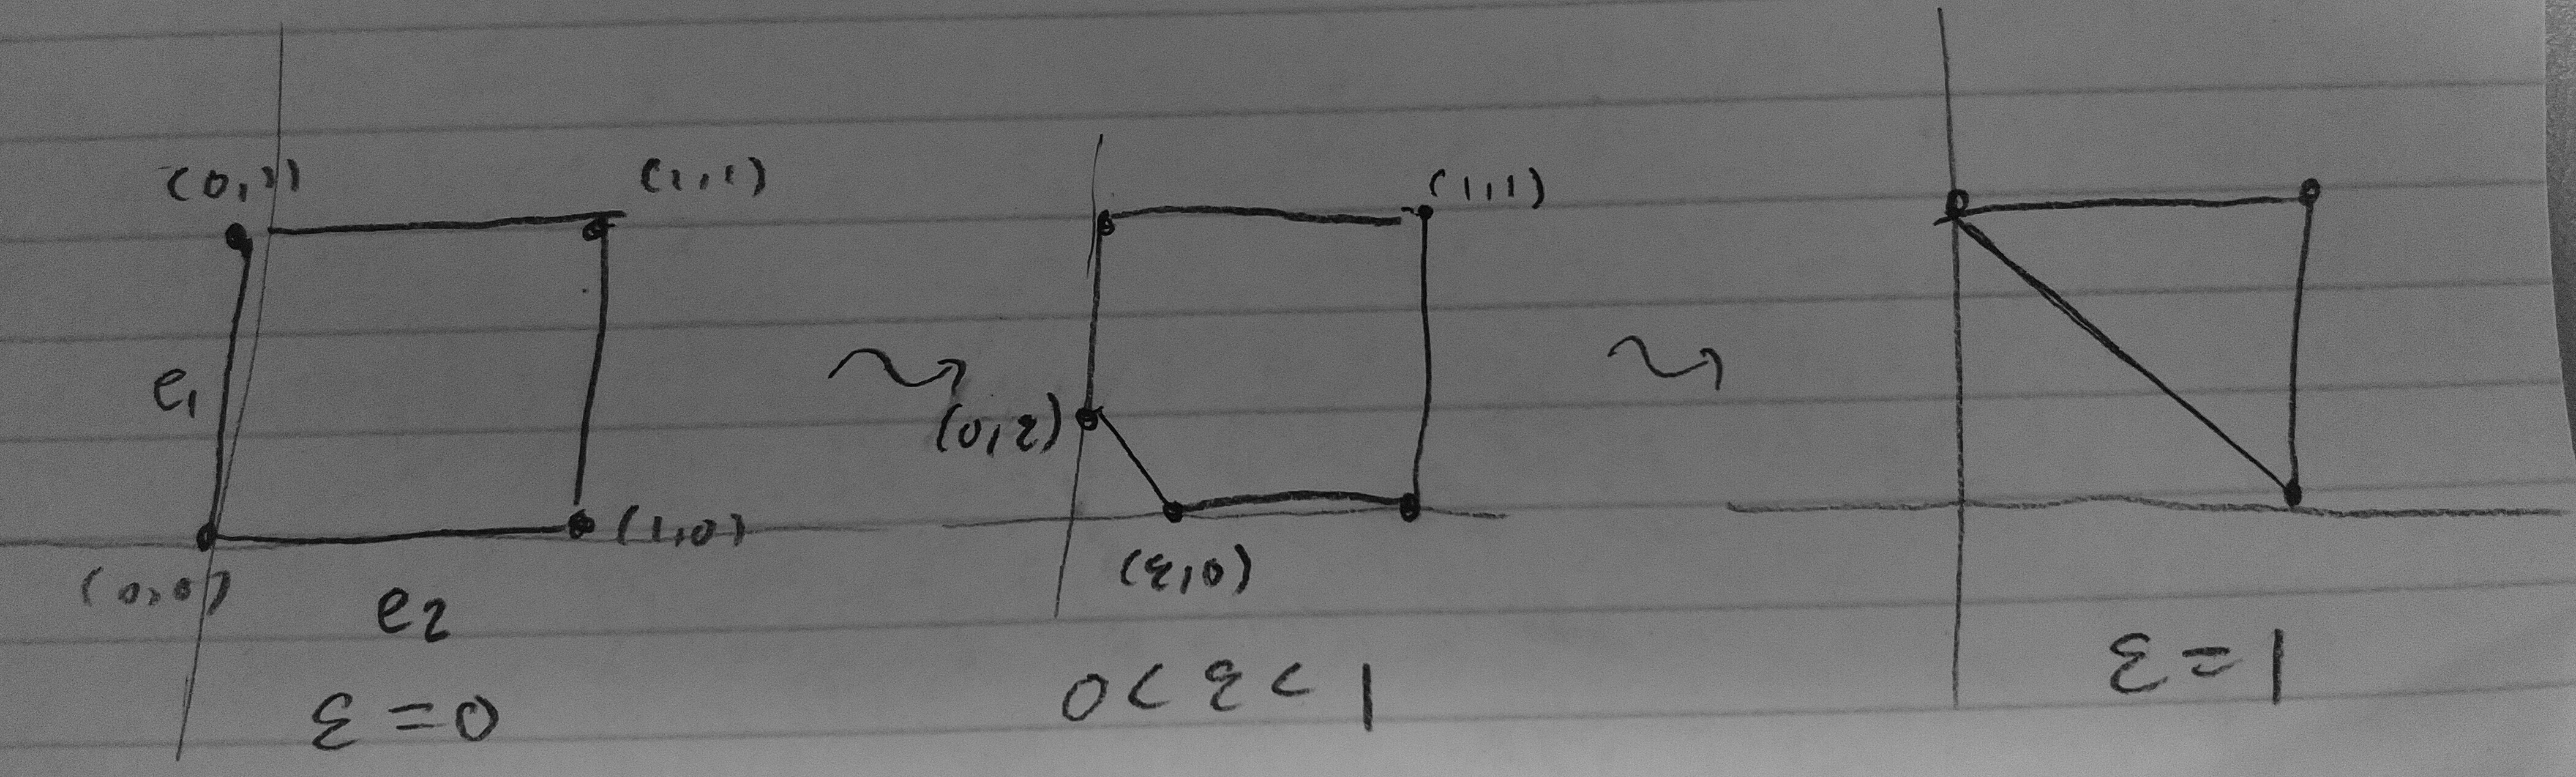
\includegraphics[width=0.8\linewidth]{polytope.jpg}
	\end{figure}
	Let $v$ denote the vertex $(0,0)$ in the bottom left. Let $\sigma$ denote the open affine associated to $v$. When $\epsilon=0$, $U_\sigma=\Spec(\C[x,y])=\C^2$. For $0<\epsilon<1$, as we analysed above we get that $X_\epsilon$ will have a blow up at the origin. Finally at $\epsilon=1$ we obtain the polytope corresponding to the toric variety $\mathbb{P}^2$. How can we interpret this? \vspace{1em}

	For each value of $\epsilon$, we have an inclusion map $\iota:P_\epsilon \to P_0$. This inclusion induces a toric morphism $X_\epsilon \to X_0$. Thus we can image $X_\epsilon$ as a $[0,1]$-family of schemes over $X_0$. For small $\epsilon$, the $X_\epsilon$ are all isomorphic, and so the $\epsilon$ data is lost. In fact for $\epsilon'>\epsilon$ we have a morphism $X_{\epsilon'}\to X_{\epsilon}$, so I imagine that as $\epsilon$ increases we are blowing up ""more"", in some vague sense.
\pagebreak

%%
%%QUESTION 4
%%
\noindent \textbf{Question 4} \\
Suppose $X_1$ and $X_2$ are two smooth toric varieties, given by the GIT data $\C^{m_1}, (\C^\ast)^{k_1}, (A_1, \omega_1)$ and $\C^{m_2}, (\C^\ast)^{k_2}, (A_2, \omega_2)$ respectively. Let $P_i, \Sigma_i$ denote their respective polytopes and fans. Further let $\{\rho_i^j\}$ denote the set of rays defining the cones in $\Sigma_i$. Then I claim that we can let $n=m_1+m_2$, $k=k_1+k_2$ and $A:\Z^n \to \Z^k$ be given by $A_1\oplus A_2$, $\omega = (\omega_1,\omega_2)$ be GIT data which will yield $X_1\times X_2$. \vspace*{1em}

$A$ defines an exact sequence (top row), taking Gale dual and $\otimes \R$ yields the bottom row.
\[\begin{tikzcd}
	M & {\Z^{n}} & {\Z^k} \\
	{\R^k} & {\R^n} & {M_\R^\vee}
	\arrow[hook, from=1-1, to=1-2]
	\arrow["{A_1\oplus A_2}", two heads, from=1-2, to=1-3]
	\arrow[Rightarrow, from=1-2, to=2-2]
	\arrow[hook, from=2-1, to=2-2]
	\arrow["{(B_1\oplus B_2)^T}"', two heads, from=2-2, to=2-3]
\end{tikzcd}\]
Letting $\rho_i$ be the image of the standard basis vector $e_i \in \R^n$, and $m_i = n_i-k_i$, we have that
$$\rho_i = \begin{cases}
    (\rho^1_i, \vec{0}_{m_2}) & i\in \{1,...,m_1\}\\
    (\vec{0}_{m_1}, \rho^2_{i-m_1}), & i\in\{m_1+1,...,m\} 
\end{cases}$$
To build the fan corresponding to this combined GIT data, we need to find the set of anticones $\cA_\omega$. For any $I\subset [m]=[m_1+m_2]$, let $I_1 = I\cap\{1,...,m_1\}$ and $I_2 = I\cap\{m_1+1,...,m\}$. Then I claim that the set of anticones is 
$$\cA_\omega = \{I_1 \cup I_2, ~|~ I_1 \in \cA^1_{\omega}, I_2 \in \cA^{2}_\omega \}.$$
This is because we can write $M_\R^\vee$ as $(M_1)_\R^\vee \oplus (M_2)_\R^\vee$ with $M_i = (\Z^{n_i - k_i})$, our stability condition also splits along this decomposition, and we have that the rays $\rho_i$ in the secondary fan also split into the rays of $X_1$ and $X_2$'s secondary fans. Finally, note that for $I = I_1\cup I_2$ in $\mathcal{A}_\omega$ we have
$$\sigma_I = \left\{\sum_{i\in I} a_i \rho_i ~|~ a_i>0 \in \mathbb{Q} \right\} = \left\{\sum_{i\in I_1}a_i \rho_i + \sum_{i\in I_2}b_i\rho_i ~|~ a_i,b_i>0\in\mathbb{Q}\right\} = \sigma_{I_1} \oplus \sigma_{I_2}.$$
Therefore we have that 
$$\Sigma_{X_1\times X_2} = \Sigma_1 \oplus \Sigma_2 := \{\sigma \oplus \tau ~|~ \sigma \in \Sigma_1, \tau \in \Sigma_2\}.$$
For the polytope, the polytope $P_i$ is defined by vertices $v^j_i$. These vertices correspond to highest-dimensional fans in $\Sigma_i$. The highest dimensional fans of $\Sigma_{X_1\times X_2}$ are sums of the highest dimensional fans of $\Sigma_1$ and those of $\Sigma_2$. If $\sigma \in \Sigma_1$ has rays $\{\rho_i\}$ and $\tau \in \Sigma_2$ has rays $\{\gamma_i\}$, then the rays in $\sigma\oplus\tau$ are $\{\rho_i+\gamma_j\}$. Let $v$,$w$ be vertices of $P_1$ and $P_2$ corresponding to $\sigma$ and $\tau$, and let $v\oplus w = (v,w)$ in $M_\R^\vee$. Then the inward facing vectors defining $v\oplus w$ are exactly the rays $\{\rho_i+\gamma_j\}$ defining $\sigma\oplus \tau$. Thus, $P_{X_1\times X_2}$ is the convex hull of the points 
$\left\{
v\oplus w ~|~ v \text{ a vertex of }P_1, w \text{ a vertex of }P_2
\right\}$.
 
\end{document}